\documentclass{article}
\usepackage[utf8]{inputenc}
\usepackage{amsmath,amssymb,amsthm}
\usepackage{graphicx}
\usepackage{wrapfig}
\graphicspath{dir=.}
\author{Nima Poshtiban}
\date{\today}
\title{Math Formulas Part 1}
\begin{document}


	\maketitle
\tableofcontents
\listoffigures
\section{Intro}

Inline Math $f\left(x\right) = 5x \cdot 3$.\newline It is obvious that
$2 + 2 \neq  5$.\newline This equation has no real answer $ x = \sqrt{-1}$

\section{Greek letters}
This is a famous equation $e^{i\pi} + 1 = 0$\newline
This is the formula of frequency \[\lambda = \frac{f}{m}\] % using display math
This is how to calculate the pressure $\rho = rgh$\newline
This is the formula of geometric progression \[
	a_{n} = a_{1} \cdot r^{n-1}
\]
\section{Trig functions}
This is the definition of hyperbolic sin \[
\sinh(x) = \frac{e^{x}-e^{-x}}{e^{x}}
\]
\begin{figure} % ---- image env
\centering

	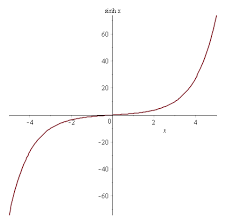
\includegraphics[scale=0.9]{sinhx.png} % --- including picture
\caption{The graph of the $\sinh(x)$}
\end{figure}
% ----  end of image env
This is an important equation
\[
\cos(x)^{2} + \sin(x)^{2} = 1
\]

%---- another way of orginazing a picture using wrapfig package
\begin{wrapfigure}{t!}{0.9\textwidth}
	\centering
	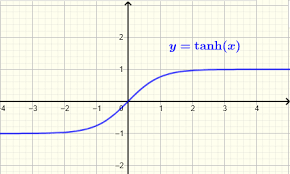
\includegraphics[]{tanhx.png}
	\caption{This is the graph of $\tanh(x)$}
\end{wrapfigure}
\end{document}